\section{aTag Enhancements}
We have demonstrated a tag format consisting of an attribute superset identifier and an bitmask, and presented algorithms for constructing such tags from an input list of attribute sets. However, we can do better.


\subsection{Variable Length Identifiers}
It is unlikely that all attribute supersets will be the same width, causing different tags to use a different number of bits. If we are using a fixed-width field in the packet headers for the tags, then it must be at least the size of the largest tag, and all smaller tags must be padded to the size of the largest tag. This wastes space which could perhaps be used in a more clever fashion.

\begin{figure}[t!] 
\begin{minipage}{1\linewidth}
\begin{subfigure}[c]{0.96\linewidth}
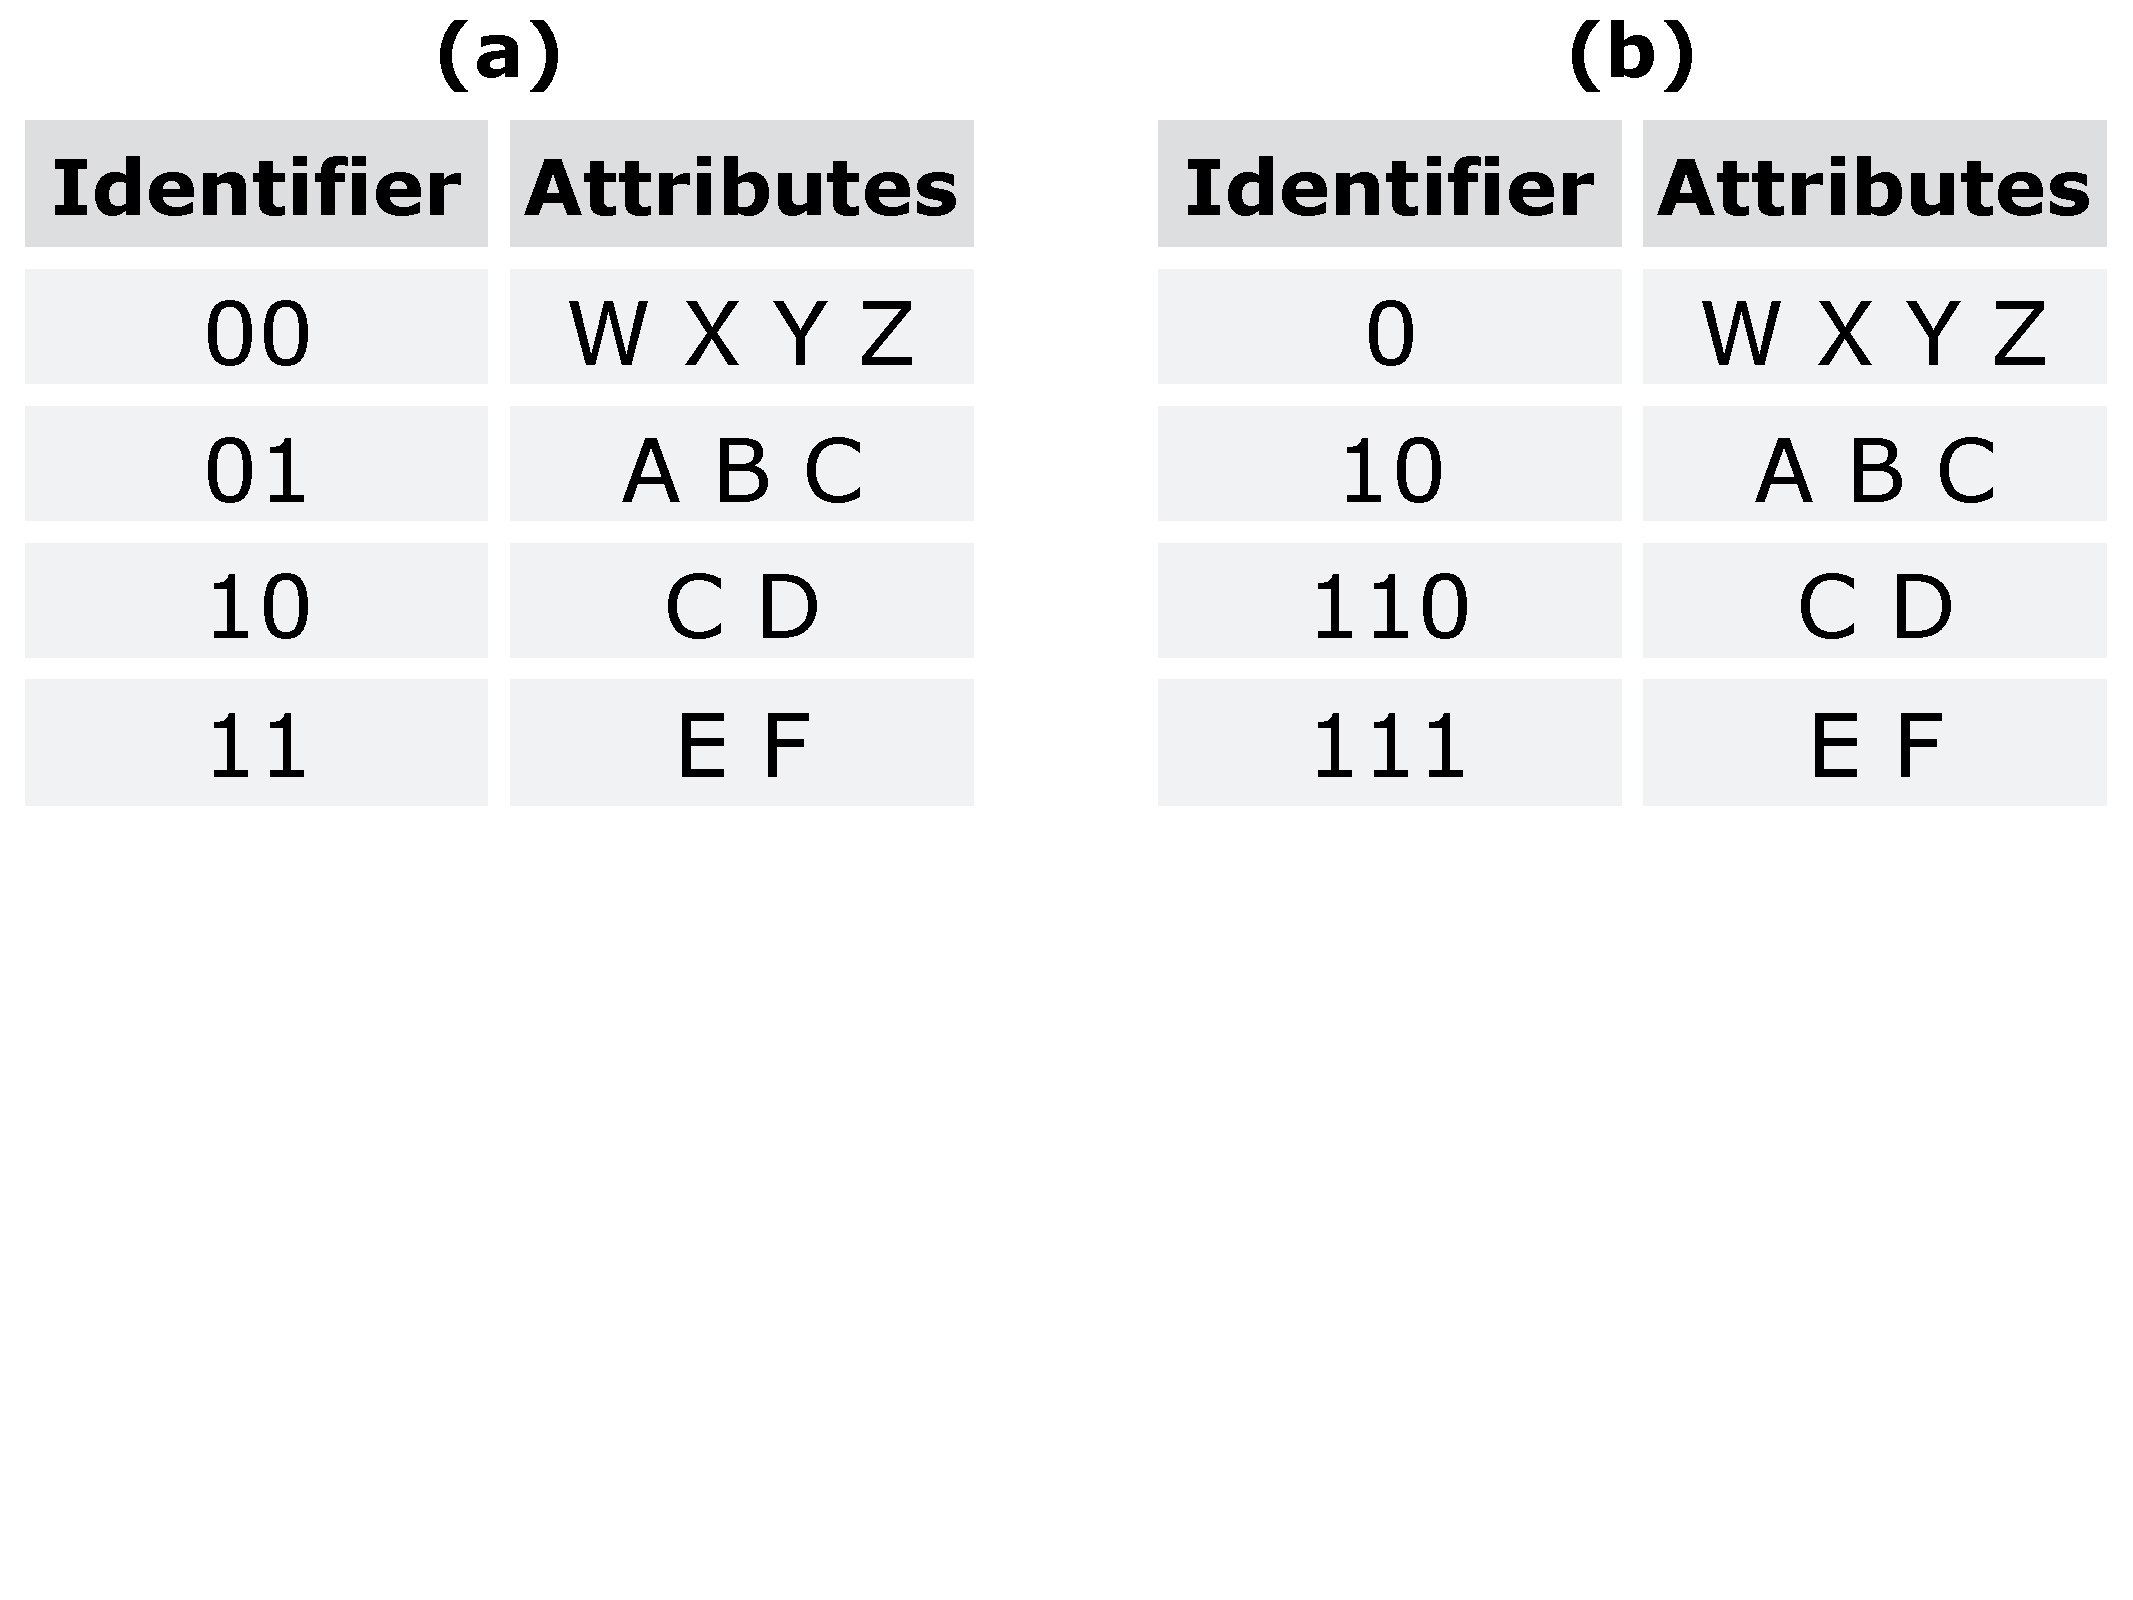
\includegraphics[trim={0 10cm 0 0}, clip, width=\linewidth]{figures/variable_identifiers}
\end{subfigure} 
\end{minipage} 
\caption{(a) shows example supersets with fixed-length identifiers. (b) shows the same supersets with variable-length identifiers. With variable length identifiers, the maximum tag width is reduced from 6 to 5 bits. }
\label{fig:variable_id}
\end{figure}

Figure \ref{fig:variable_id}(a) shows an example list of supersets, where the tag width is determined by one large superset. If the largest superset had a smaller identifier, the tag width could be decreased. We can accomplish this with the use of prefix codes. A prefix code is a set of (not necessarily equal-length) identifiers such that no identifier is a prefix of any other identifier. Figure \ref{fig:variable_id}(b) shows an example prefix code identifier assignment, which decreases the overall tag width from 6 bits to 5 bits.






\subsection{Encoding Total and Partial Orderings}
In the design of our tag format, we assumed that the attribute sets to encode have no ordering: no attribute is greater or less than any other attribute. In many cases, this is true, as in the example of encoding lists of next-hops, but this is not true for all applications. For the example of encoding paths of middleboxes, the middleboxes must be traversed in the order originally specified. As our scheme currently stands, this ordering is lost after the sequence is converted to a tag. 

\subsubsection{Total Ordering}
It is possible to impose an ordering upon the elements encoded by the tags. If the forwarding table entries which test for element membership were prioritized such that testing for element $X$ always has higher priority than testing for element $Y$, then this imposes the ordering $X > Y$ on the pair. Forwarding tables return the highest priority match, so if both $X$ and $Y$ are present in the sequence, then the test for $X$ will be the test that returns true. We can use this idea to support element ordering, so long as the element set is \textit{totally ordered}.

\subsubsection{Partial Ordering}
It may not always be the case that the attributes have a total ordering, but it may be nearly the case for some applications. If, across all sequences, there are a few pairs of attributes $X$ and $Y$ such that $X$ appears before $Y$ in some sequences and $Y$ appears before $X$ in others, then $X$ and $Y$ are incomparable and we say that the universe is \textit{partially ordered}. It is still possible to encode such a list of sequences using our scheme, but at the cost of slightly larger tags.

Support for partial orderings is possible with one key observation: for a sequence to be ordered, switches must be able to perform ordered membership testing. If we have elements $[X,Y,Z]$ with $X > Y > Z$, then membership of $X$ is tested first by checking for for the $X$ bit, then $Y$, and finally $Z$. If however, we had to encode the two paths $XYZ$ and $YXZ$, this approach fails when each element is mapped to only one bit. Were we to map $X$ to two bits, one before $Y$ and one after $Y$, then $XYZ$ could be encoded as $1101$ and $YXZ$ would be $0111$. The bits could be tested in order from left to right, and both paths would be recreated correctly. 

To convert from a partial ordering to a totally ordered sequence of bits, incomparable pairs of elements could be made comparable by \textit{splitting} of one of the bits. For example, consider an incomparable pair $(B, C)$. We could split $B$ into bits $B_1$ and $B_2$. In every order where $B$ appears before $C$, we would replace $B$ with $B_1$. When $B$ appears after $C$, we would use $B_2$. This creates the ordering $B_1 < C < B_2$, resolving the incomparability! If every pair of incomparable elements is resolved with splitting, then the partially ordered universe of elements is replaced by a totally ordered new, larger universe of elements, where each element in the new universe can be mapped to an element in the original universe. We can then use this new universe to create tags for each sequence. 